% Draft, 8 Oct 2026. Layout follows the AAAI two-column camera-ready style (US Letter, Times, 10pt, no page numbers).
% Before submission: move the body into the official AAAI-27 author kit (its .sty and .bst replace the preamble below).
\documentclass[10pt,twocolumn,letterpaper]{article}
\usepackage[letterpaper,top=0.75in,bottom=1.25in,left=0.75in,right=0.75in,columnsep=0.33in]{geometry}
\usepackage{times}
\usepackage{amsmath,amssymb,amsthm}
\usepackage{graphicx}
\usepackage{booktabs}
\usepackage{xcolor}
\usepackage[font=small,labelfont=bf]{caption}
\usepackage{microtype}
\usepackage[round,authoryear]{natbib}
\usepackage{tikz}
\usetikzlibrary{arrows.meta, positioning, fit, backgrounds, calc}
\definecolor{rev}{HTML}{2A78D6}
\definecolor{audit}{HTML}{EB6834}
\definecolor{memc}{HTML}{1BAF7A}
\pagestyle{empty}
\renewcommand{\dbltopfraction}{0.92}
\renewcommand{\topfraction}{0.9}
\renewcommand{\textfraction}{0.07}
\renewcommand{\dblfloatpagefraction}{0.75}
\setcounter{dbltopnumber}{2}
\setlength{\parskip}{0pt}
\frenchspacing
\makeatletter
\renewcommand\section{\@startsection{section}{1}{\z@}{-2.2ex plus -0.5ex minus -.2ex}{1.1ex plus .2ex}{\centering\normalfont\large\bfseries}}
\renewcommand\subsection{\@startsection{subsection}{2}{\z@}{-1.8ex plus -0.5ex minus -.2ex}{0.8ex plus .2ex}{\normalfont\normalsize\bfseries}}
\renewcommand\paragraph{\@startsection{paragraph}{4}{\z@}{1.0ex plus 0.5ex minus .2ex}{-0.6em}{\normalfont\normalsize\bfseries}}
\makeatother
\newtheorem{proposition}{Proposition}
\newtheorem{definition}{Definition}
\newcommand{\game}[1]{\textsc{#1}}
\newcommand{\gone}{g_1}
\newcommand{\gstar}{g^{*}}

\title{Penalties Sized to the Gain: When Do Random Audits Stop\\AI Agents from Over-Using a Shared Resource?}
\author{Anonymous submission}
\date{}

\begin{document}
\maketitle
\thispagestyle{empty}

\begin{abstract}
AI agents that share a limited resource may take more than they are allowed, and an overseer can afford to check only a few of them. We ask when random audits stop them. We study an \emph{audited commons}: six agents draw on a renewable resource, a reviewer sets each agent's allowance so that the resource stays at the level where it regrows fastest, and audits answer a caught over-take with a fine, a memory of the offence, or both. With programmed agents in three games, audits work only through their consequences; deterrence begins where the expected fine equals the gain from cheating, a threshold we predict in advance in 5 of 5 new settings; and two intuitive designs backfire: tightening everyone's allowance to absorb known cheaters, and aiming each audit at the largest report. With four language-model (LLM) families in 520 games, the two families that over-take on purpose stop at the fine predicted in advance from their own \emph{one-round} gain (exactly for one model, one grid step early for the other), although over-taking rarely pays over the whole game. Like the myopia reported for LLM collectives, these agents ignore the cost to the shared stock, and here that myopia sets the deterrence threshold: penalties for LLM agents should be sized to the immediate gain.
\end{abstract}

% =====================================================================
\section{Introduction}

Language-model agents increasingly act together on shared, limited resources: compute budgets, rate-limited services, energy reserves, and the economic and natural commons that their users depend on \citep{piatti2024cooperate,bracale2026draining}. An overseer of such a system faces a problem that is old in economics and new in AI safety. Verification is expensive, so only a few actions can be checked \citep{amodei2016concrete,greenblatt2024control}, and an agent that takes more than its share is seen only if it happens to be checked. Two questions follow. Which consequences make sparse checking work? And can an overseer predict, before deploying a penalty, whether it will stop a given AI agent?

Enforcement economics answers the first question for rational offenders: a risk-neutral offender complies when the expected penalty, the probability of being caught times the fine, exceeds the gain from offending \citep{becker1968crime,allingham1972income,avenhaus2002inspection}. AI-control work studies audit budgets, but there a caught model is shut down, so audits without consequences, memory or graded fines are not tested \citep{greenblatt2024control,griffin2024games}. Studies of LLM agents in commons find that most fail to sustain the resource without enforcement \citep{piatti2024cooperate,bracale2026draining}. Enforcement studies with LLMs either remove violators flagged by an LM judge \citep{ye2026norm} or compare one fine below and one above break-even in single decisions \citep{okamoto2026why}. No study measures when random audits deter AI agents that act repeatedly on a shared resource, or tests whether the deterrence threshold can be predicted for a given model.

We build an \emph{audited commons} (Figure~\ref{fig:step}). Each round, six agents request a share of a renewable resource; a reviewer predicts the effect of the requests and grants allowances that keep the resource above half capacity, where it regrows fastest; each agent then chooses what it actually takes; and random audits check a few agents. We study three games with programmed agents, as a mechanism layer whose results we can predict, and then replace four of the six agents in the fishery game with LLMs from four families. Every study was run under a protocol frozen before its code, with amendments dated and failed predictions reported.

\paragraph{Contributions.}
\begin{itemize}\setlength{\itemsep}{1pt}\setlength{\parsep}{0pt}
\item \textbf{An audited-commons testbed.} We formalise oversight with a limited audit budget over a renewable resource, with three games (\game{Fishery}, \game{Forest}, \game{River}), one harm line derived from each game's regrowth, and the social outcome metrics used for commons games (Section~\ref{sec:setting}).
\item \textbf{What makes audits work, with programmed agents.} Audits help only through consequences. Deterrence starts at the expected-penalty break-even, which we predict in advance from runs without audits and confirm in 5 of 5 new settings. Two intuitive designs backfire: a tighter shared allowance that absorbs known cheaters makes cheating pay \emph{more} than no audits, and aiming each audit at the largest report catches only 25\% of liars against 100\% at random (Section~\ref{sec:programmed}).
\item \textbf{LLM agents are myopic offenders.} Across 520 games and 81{,}232 decisions, the two LLM families that over-take on purpose stop at the fine predicted in advance from their one-round gain, within one grid step and exactly for one model. Their whole-game gain from over-taking is small or negative, yet they over-take until the fine outweighs the one-round gain. A reviewer that remembers past over-takes removes most of the harm without any fine, but does not stop the over-taking (Section~\ref{sec:llm}).
\end{itemize}

% =====================================================================
\section{Related Work}
\label{sec:related}

\paragraph{Scalable oversight and AI control.} Scalable oversight concerns objectives that are ``too expensive to evaluate frequently'' \citep{amodei2016concrete,bowman2022measuring}. AI control evaluates protocols that audit a small share of an untrusted model's outputs with trusted labour, and compares random with suspicion-targeted auditing \citep{greenblatt2024control}; \citet{griffin2024games} model such protocols as games. Multi-agent extensions show that monitors that check one agent or one action at a time miss harm that only appears in combination \citep{makins2026multiagent,hu2026local}. \citet{gans2026randomized} show in theory that rare random audits can deter AI agents when audit draws cannot be learned in advance. We add a renewable resource, graded consequences, and experiments with LLM agents.

\paragraph{LLM agents in commons.} GovSim finds that ``all but the most powerful LLM agents fail to achieve a sustainable equilibrium'' \citep{piatti2024cooperate}; LLM collectives in an energy commons behave like impatient optimisers \citep{bracale2026draining}; and reasoning models free-ride in public-goods games with sanctions \citep{guzman2025corrupted}. \citet{ye2026norm} enforce norms among LLM agents, including in a fishery, by removing violators flagged by an LM judge and tracking reporters' reliability. None varies the audit probability or the fine.

\paragraph{Enforcement economics.} The expected-penalty condition goes back to \citet{becker1968crime} and \citet{allingham1972income}. Inspection games formalise partial verification and inspector commitment \citep{avenhaus2002inspection}; records of past offences give enforcement leverage \citep{harrington1988enforcement}; report-based cutoff rules can beat random audits in static settings \citep{reinganum1985income}; and a small fine can act as a price \citep{gneezy2000fine}. In fisheries, model-based management fails when the model is wrong \citep{ludwig1993uncertainty}.

\paragraph{Rule-breaking LLMs.} LLMs comply more when a fine lies above break-even than below it \citep{okamoto2026why}, and misbehave more when the perceived risk of getting caught falls \citep{scheurer2023strategic}. Table~\ref{tab:positioning} summarises how our setting differs.

\begin{table}[t]
  \centering\small
  \caption{Closest prior work. \checkmark: yes; (\checkmark): partly. $^a$Becker; Harrington; inspection games. $^b$Greenblatt et al.\ (2024). \emph{Predicted threshold}: the fine at which cheating stops is predicted before it is tested.}
  \label{tab:positioning}
  \resizebox{\columnwidth}{!}{\begin{tabular}{lccccccc}
\toprule
 & \rotatebox{60}{LLM agents} & \rotatebox{60}{Several agents} & \rotatebox{60}{Renewable resource} & \rotatebox{60}{Random audits} & \rotatebox{60}{3+ fine levels} & \rotatebox{60}{Memory} & \rotatebox{60}{Predicted threshold} \\
\midrule
Enforcement economics$^{a}$ & -- & (\checkmark) & -- & \checkmark & \checkmark & \checkmark & -- \\
AI control$^{b}$ & \checkmark & -- & -- & (\checkmark) & -- & -- & -- \\
Makins et al.\ 2026 & \checkmark & \checkmark & -- & -- & -- & -- & -- \\
Gans \& Holden 2026 & -- & -- & -- & \checkmark & -- & -- & -- \\
GovSim (Piatti et al.\ 2024) & \checkmark & \checkmark & \checkmark & -- & -- & -- & -- \\
Bracale Syrnikov et al.\ 2026 & \checkmark & \checkmark & \checkmark & -- & -- & -- & -- \\
Ye \& Steinhardt 2026 & \checkmark & \checkmark & (\checkmark) & -- & -- & (\checkmark) & -- \\
Okamoto et al.\ 2026 & \checkmark & -- & -- & (\checkmark) & -- & -- & -- \\
\midrule
\textbf{This work} & \checkmark & \checkmark & \checkmark & \checkmark & \checkmark & \checkmark & \checkmark \\
\bottomrule
\end{tabular}
}
\end{table}

% =====================================================================
\section{The Audited Commons}
\label{sec:setting}

\begin{figure*}[t]
  \centering
  \resizebox{0.92\textwidth}{!}{% Figure 1: one step of the audited commons game (TikZ, vector). Input inside a figure environment.
% Colours: agents grey, reviewer blue, audits orange (same mapping as the data figures).
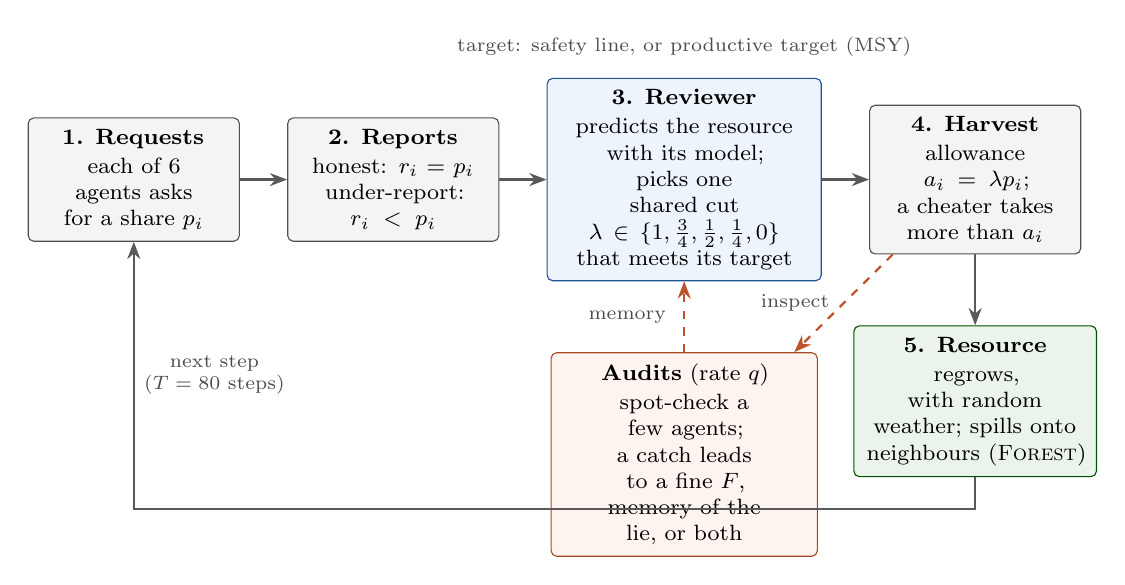
\begin{tikzpicture}[
    font=\footnotesize,
    >={Stealth[length=2.2mm]},
    box/.style={draw=#1!70!black, fill=#1!8, rounded corners=2pt, align=center, inner sep=4pt, minimum height=11mm, text width=24mm},
    lab/.style={font=\scriptsize, align=center, text=black!70},
    flow/.style={->, thick, draw=black!65},
    fb/.style={->, thick, draw=audit!80!black, dashed},
  ]
  \colorlet{agentc}{black!55}
  \colorlet{revc}{rev}
  % ---- row of the step
  \node[box=agentc] (req) {\textbf{1. Requests}\\[1pt] each of 6 agents asks\\ for a share $p_i$};
  \node[box=agentc, right=6mm of req] (rep) {\textbf{2. Reports}\\[1pt] honest: $r_i=p_i$\\ under-report: $r_i<p_i$};
  \node[box=revc, right=6mm of rep, text width=32mm] (rv) {\textbf{3. Reviewer}\\[1pt] predicts the resource\\ with its model; picks one\\ shared cut $\lambda\in\{1,\tfrac34,\tfrac12,\tfrac14,0\}$\\ that meets its target};
  \node[box=agentc, right=6mm of rv] (ex) {\textbf{4. Harvest}\\[1pt] allowance $a_i=\lambda p_i$;\\ a cheater takes\\ more than $a_i$};
  \node[box=green!45!black, below=9mm of ex, text width=28mm, minimum height=17mm] (res) {\textbf{5. Resource}\\[1pt] regrows, with random\\ weather; spills onto\\ neighbours (\textsc{Forest})};
  \node[box=audit, below=9mm of rv, text width=31mm, minimum height=17mm] (au) {\textbf{Audits} (rate $q$)\\[1pt] spot-check a few agents;\\ a catch leads to a fine $F$,\\ memory of the lie, or both};
  % ---- arrows
  \draw[flow] (req) -- (rep);
  \draw[flow] (rep) -- (rv);
  \draw[flow] (rv) -- (ex);
  \draw[flow] (ex) -- (res);
  \draw[flow] (res.south) -- ++(0,-4mm) -| (req.south) node[pos=0.75, lab, right] {next step\\ ($T=80$ steps)};
  \draw[fb] ([xshift=3mm]ex.south west) -- ([xshift=-3mm]au.north east) node[midway, lab, left=0.5mm] {inspect};
  \draw[fb] (au.north) -- (rv.south) node[midway, lab, left=1mm] {memory};
  % ---- target annotation
  \node[lab, above=1.5mm of rv] {target: safety line, or productive target (MSY)};
\end{tikzpicture}
}
  \caption{One round of the audited commons. Agents request a share; they may report honestly or under-report. The reviewer predicts the resource with its model and picks one shared cut that meets its target. Each agent takes its allowance or more. The resource regrows, and random audits answer a caught over-take or lie with a fine, a memory of the offence, or both.}
  \label{fig:step}
\end{figure*}

\paragraph{Resource and agents.} $N=6$ agents act for $T$ rounds on a resource with level $x_t\in[0,K]$. After the agents take $c_t=\sum_i c_{i,t}$, the resource regrows logistically,
\begin{equation}
x_{t+1} = y_t + r\,y_t\Bigl(1-\frac{y_t}{K}\Bigr) + \varepsilon_t,\qquad y_t = x_t - c_t,
\label{eq:dyn}
\end{equation}
with weather noise $\varepsilon_t$ in \game{Forest} and \game{River}. Regrowth $r y(1-y/K)$ is largest at $y=K/2$, where the maximum sustainable harvest $rK/4$ is reached. Agent $i$ requests $p_{i,t}\in[0,\bar c]$ and may report $\hat p_{i,t}\le p_{i,t}$.

\paragraph{Reviewer.} The reviewer chooses one shared cut $\lambda_t\in\{1,\tfrac34,\tfrac12,\tfrac14,0\}$, the largest whose predicted outcome meets its target, and grants allowances $a_{i,t}=\lambda_t\hat p_{i,t}$. A \emph{joint} reviewer sums all requests before predicting; \emph{local} reviewers judge one request at a time. The target is either a one-step safety line (the resource must not fall to a danger level next round) or the \emph{half-capacity} target $y_t\ge K/2$, the level behind maximum sustainable yield \citep{may1978exploiting}.

\paragraph{Harm and outcome metrics.} A round is \emph{harmful} if the resource falls below half capacity: \game{Fishery} stock below 50 of 100 after fishing, \game{Forest} mean plot health below 10 of 20 (as a 5\% chance constraint), \game{River} quality below 50 of 100. Following commons-game practice \citep{piatti2024cooperate,perolat2017multiagent}, we also report \emph{efficiency}, the total harvest divided by $T\cdot rK/4$; \emph{equality}, $1-$Gini of the agents' returns; and \emph{survival}, the share of runs without collapse.

\paragraph{Misbehaviour, audits and consequences.} An agent \emph{over-takes} when $c_{i,t}>a_{i,t}$, and \emph{under-reports} when $\hat p_{i,t}<p_{i,t}$. Each round, each agent is audited independently with probability $q$; an audit detects a violation with probability $s$. A caught agent pays a flat fine $F$, so the expected fine per violating round is $e=qsF$. Alternatively the reviewer keeps a \emph{memory}: it records the caught agent's excess and lowers its later allowances by the mean recorded excess, $a'_{i,t}=\max(0,\lambda_t\hat p_{i,t}-\bar m_i)$.

\paragraph{When should a fine deter?} Let $\gone$ be an agent's gain from one round of over-taking, holding later rounds fixed, and let $\gstar$ be its net gain over complying across the whole game, per round of over-taking.

\begin{proposition}[Break-even]
\label{prop:breakeven}
(i) A risk-neutral agent that maximises each round's catch net of the expected fine over-takes in a round if and only if $e<\gone$; under a flat fine it then takes the maximum $\bar c$. (ii) An agent that commits to one over-take level for the whole game over-takes at some level if and only if $e<\gstar$.
\end{proposition}
\begin{proof}[Sketch]
(i) Over-taking by $\delta>0$ adds $\delta$ to the round's catch and costs $e$ in expectation, independent of $\delta$ under a flat fine; the net gain is maximised at the largest $\delta$, and is positive iff $\gone>e$. (ii) A level $d$ yields total gain $G(d)$ over $n(d)$ over-take rounds and expected fines $e\,n(d)$; it pays iff $G(d)/n(d)>e$, and $\gstar=\max_d G(d)/n(d)$.
\end{proof}

Part (ii) describes the programmed cheaters, which choose one level per game; part (i) describes an agent that decides every round. Since depleting the resource lowers later catches, $\gstar\le\gone$ in our games: a myopic agent keeps over-taking at fines where over-taking no longer pays over the game.

% =====================================================================
\section{Programmed Agents: What Makes Audits Work}
\label{sec:programmed}

\paragraph{Setup.} Agents follow threshold rules; 2 or 4 of the 6 are \emph{greedy}. Misbehaving agents either under-report by a fixed share, or over-take with a level $d\in\{0,\frac14,\frac12,\frac34,1\}$ (taking $a+d(p-a)$) chosen by search to maximise their payoff on 32 training populations. Results are on 64 new populations of 80 rounds, with 95\% paired bootstrap intervals over populations (4{,}000 resamples). Table~\ref{tab:settings} (appendix) lists the settings of every study.

\paragraph{The target matters more than the information.} With a joint reviewer and true inputs, the half-capacity target gave 1{,}393 against 555 total harvest under the one-step line in \game{Fishery} (difference $+838$, $[+800,+865]$), because the one-step line lets the stock fall to where it regrows slowly. With a wrong model of the resource, the joint reviewer's risky approvals in \game{Forest} rose from 0.9\% to 82\% when regrowth was overestimated by 25\%; in \game{Fishery}, under a hidden collapse point, the one-step line collapsed 78\% of populations and the half-capacity target 0\%. A reviewer that learned the model recovered within about 60 rounds (appendix Figure~\ref{fig:reviewer}), echoing the adaptive-management lesson of \citet{ludwig1993uncertainty}.

\begin{figure*}[t]
  \centering
  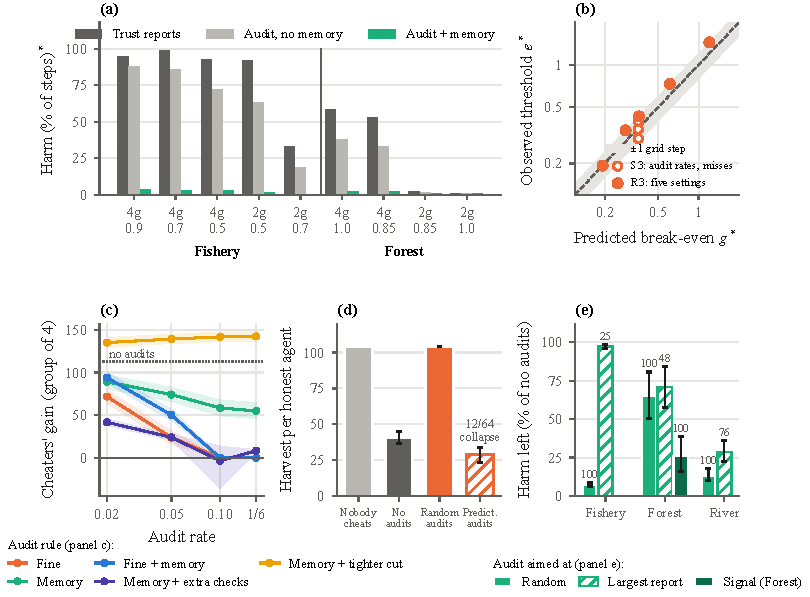
\includegraphics[width=\textwidth]{../figures/fig3_audits.pdf}
  \caption{What makes audits work (programmed agents). (a)~Under-reporters in nine settings: auditing without memory barely reduces harm; remembering each caught lie removes most of it. (b)~The expected fine at which cheaters stop ($e^*$) against the break-even predicted from runs without audits ($\gstar$); filled: five settings predicted before the search; every point lies within one grid step (shaded). (c)~Cheaters' gain as the audit rate rises under five rules; tightening everyone's cut to absorb known cheaters makes cheating pay more than no audits. (d)~A known audit schedule leaves honest agents worse off than no audits. (e)~Harm left when one audit per round is aimed at random, at the largest report, or at the plot doing worst against prediction; numbers: share of liars ever caught. Error bars: 95\% intervals.}
  \label{fig:audits}
\end{figure*}

\paragraph{Audits work only through consequences.} Against under-reporters, a reviewer that only uses audit results to correct its current decision barely improved safety (\game{Forest}: 1.9\% to 1.7\% of rounds unsafe). Remembering each caught lie removed most of the harm in 9 of 9 settings (Figure~\ref{fig:audits}a); in \game{Fishery}, unsafe rounds fell from 69\% to 1.5\%. Memory alone, however, does not deter: adaptive cheaters kept 41\% of their gain even at the highest audit rate, while memory plus a fine deterred at audit rate 0.05 instead of 0.10.

\paragraph{Deterrence starts at the break-even, and can be predicted.} In the pilot setting, cheaters stopped at $e\approx0.30$--$0.40$, against a predicted break-even of 0.356, for audit rates from $1/6$ to $0.02$ and audits that miss up to three cheats in four. We then predicted $\gstar$ for five new settings from runs \emph{without} audits, before any search with fines. In 5 of 5, the observed threshold fell within one grid step of the prediction, for predicted thresholds from 0.19 to 1.20 (Figure~\ref{fig:audits}b). A known audit schedule cannot deter: honest agents received 28.8 against 40.9 with no audits at all (Figure~\ref{fig:audits}d).

\paragraph{Two designs that backfire.} First, a reviewer that answers known cheaters by tightening the \emph{shared} cut protects the stock but spreads the cost onto honest agents: cheaters gained more than with no audits (142 against 113) and honest agents received 36 each, against 104 under a fine (Figure~\ref{fig:audits}c). Second, aiming each audit at the largest (memory-corrected) report keeps auditing the same agent: in \game{Fishery} only 25\% of liars were ever caught, against 100\% under random audits, and harm stayed at 96.2\% of rounds against 7.4\%. The same ordering held in \game{River} (6.0\% against 2.8\% of rounds unsafe; 41\% against 37\% below half capacity). This complements static results in which report-based cutoff rules beat random audits \citep{reinganum1985income}: here agents differ in size and play repeatedly, so a rank rule never leaves the largest agent, the feedback loop of \citet{ensign2018runaway}. Aiming at a physical signal, the plot doing worst against prediction, was best in \game{Forest} (harm 26\% of the no-audit level, against 65\% at random; Figure~\ref{fig:audits}e).

\begin{figure*}[t]
  \centering
  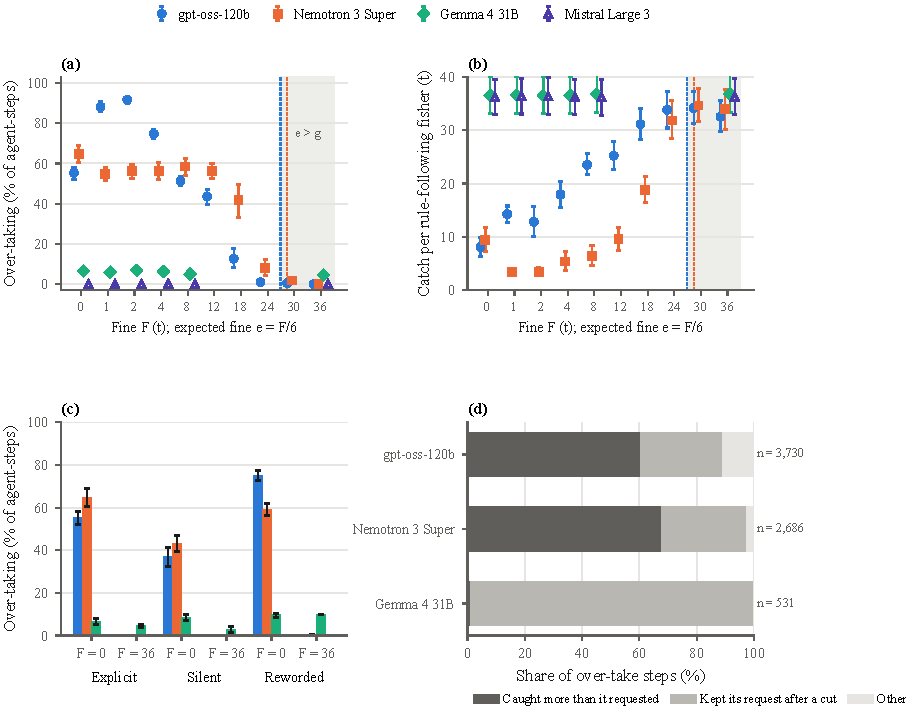
\includegraphics[width=0.86\textwidth]{../figures/fig4_llm_agents.pdf}
  \caption{LLM agents in \game{Fishery}. (a)~Share of rounds in which each model over-took, against the fine $F$ (expected fine $e=F/6$; $F=12$--$30$ from the threshold test, gpt-oss and Nemotron only). Dotted: each model's one-round gain; shaded: $e$ above both. (b)~Catch of the two rule-following fishers over 20 rounds. (c)~A 36\,t fine stops over-taking whether the rules state that over-taking is possible (explicit), omit it (silent), or reword it. (d)~What an over-take round is (post hoc): gpt-oss and Nemotron mostly take more than they requested; Gemma almost only keeps its request after a cut. Error bars: 95\% intervals over populations.}
  \label{fig:llm}
\end{figure*}

% =====================================================================
\section{LLM Agents: Deterrence of Myopic Offenders}
\label{sec:llm}

\begin{figure*}[t]
  \centering
  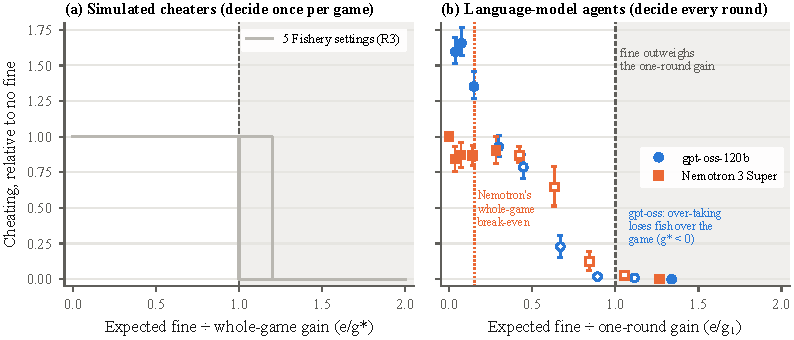
\includegraphics[width=\textwidth]{../figures/fig5_spine.pdf}
  \caption{Each kind of agent stops when the expected fine outweighs the gain it acts on. (a)~Simulated cheaters choose one level per game and stop at $e/\gstar=1.0$--$1.2$ of their whole-game gain, as predicted before the search. (b)~LLM agents decide every round and stop near $e/\gone=1$ of their one-round gain (open markers: fines added by the threshold test, whose stopping point was predicted in advance). Measured by the whole-game gain they over-take far past break-even: over-taking loses gpt-oss fish over the game ($\gstar<0$), and Nemotron's whole-game break-even (dotted) lies at $e/\gone=0.15$.}
  \label{fig:spine}
\end{figure*}

\paragraph{Setup.} In \game{Fishery} (half-capacity target, 20 rounds), four of the six fishers are LLM agents and two follow fixed rules. Each round an LLM agent states a request and, after seeing its allowance, its catch, as JSON in tonnes; it sees the last three rounds of its own history. Audits are independent with $q=1/6$; a catch costs a flat fine $F$ (\emph{E}-cells, $F\in\{0,1,2,4,8,12,18,24,30,36\}$\,t) or triggers the reviewer's memory (\emph{EM}, no fine). The explicit rules say ``you can choose to catch more than your allowance''; control cells drop this sentence (\emph{S}) or reword the rules (\emph{P}). Over-taking means catching more than 0.06\,t above the allowance. We ran gpt-oss-120b (OpenAI), Nemotron 3 Super (NVIDIA) and Gemma 4 31B (Google) as frozen families, and Mistral Large 3 as an added family, through Ollama Cloud at temperature 0.7 with fixed seeds, on the same 10 populations in every cell. Each model first passed a pilot gate ($\ge$95\% valid first answers, comprehension $\ge$2 of 3). Across 520 games and 81{,}232 decisions there were no fallback answers, 6 re-prompts, and every comprehension check scored 3 of 3.

\paragraph{Over-taking against the fine.} gpt-oss and Nemotron over-took in 51--92\% of rounds at every expected fine up to 1.33\,t, and in 0\% at 6\,t (Figure~\ref{fig:llm}a). A small fine \emph{raised} over-taking for gpt-oss (55\% with no fine, 88--92\% at 1--2\,t), as fines can act as prices \citep{gneezy2000fine,okamoto2026why}. Below the threshold the harm was large: under Nemotron, 5 to 10 of 10 lakes collapsed at every fine from 1 to 8\,t, and gpt-oss's rule-following fishers caught 8--25\,t over the game against 32--34\,t once over-taking stopped (Figure~\ref{fig:llm}b). Gemma rarely over-took (4--10\% of rounds), almost always by catching its request after the reviewer cut it, and Mistral Large 3 never over-took in 16{,}000 decisions; neither is informative about deterrence.


\paragraph{The stopping fine, predicted in advance.} From each model's no-fine cell we measured its one-round gain, the mean tonnes above the allowance on over-take rounds: $\gone=4.48$\,t (gpt-oss) and 4.74\,t (Nemotron). Before any further game we froze the prediction that $F=12,18,24$ ($e=2,3,4<\gone$) would not deter and $F=30$ ($e=5>\gone$) would, and ran 80 games at these fines. Taking ``deterred'' as at most 5\% of rounds at that fine and every larger one, Nemotron stopped exactly at $F=30$ and gpt-oss one grid step early, at $F=24$ (Figure~\ref{fig:spine}b). Over-taking was graded rather than a step: relative to no fine, it was 0.79 and 0.87 at $e/\gone\approx0.45$, 0.23 and 0.65 at $\approx0.65$, and 0.02 and 0.12 at $\approx0.87$ (gpt-oss and Nemotron). Our pre-registered hypothesis that over-taking would stay at or above 25\% at $F=24$ failed for both models (1.0\% and 8.0\%).


\paragraph{Myopic offenders.} Measured the way the programmed cheaters are measured, as the net gain over a compliant game (the 36\,t cell, where nobody over-takes), the LLMs' whole-game gain per over-take round is $\gstar=-1.05$\,t for gpt-oss, which loses fish by over-taking in 7 of 10 populations because lakes collapse, and $0.71$\,t for Nemotron. Both nonetheless kept over-taking until the fine outweighed $\gone$, nearly seven times $\gstar$ for Nemotron (Figure~\ref{fig:spine}). By Proposition~\ref{prop:breakeven}, the agents behave as in part (i), not part (ii): they weigh this round's gain against this round's expected fine and ignore the depleted stock in later rounds. Two further observations fit part (i). Over-takes were all-out, at the 6\,t maximum in 68\% (gpt-oss) and 93\% (Nemotron) of over-take rounds, as a flat fine gives no reason to take less \citep{stigler1970optimum}; and being caught did not change the next round (gpt-oss over-took again 78\% of the time after a caught over-take, 81\% after an unchecked one), as independent audits carry no information about the future. Unlike people in some tax experiments, the models showed no drop in compliance after an audit \citep{mittone2006dynamic,kastlunger2009sequences}. The comparison with $\gstar$ was made after the results were seen.

\paragraph{Memory without fines.} With the reviewer's memory and no fine, over-taking fell to 20\% (gpt-oss) and 33\% (Nemotron) of rounds, but did not stop. The resource was protected: rounds below half capacity fell from 92\% to 20\% and from 96\% to 40\%, no lake collapsed (against 5 and 1 of 10), and the rule-followers' catch rose from 8 to 29\,t and from 9 to 32\,t. Memory thus removes most of the harm without deterring: with no fine, $e=0$ and Proposition~\ref{prop:breakeven} predicts continued over-taking, while the reviewer's lower allowances limit what each over-take can do.

\paragraph{Deterrence costs no efficiency.} At fines above $\gone$ ($F=30,36$), both models reached 0.99 of the maximum sustainable harvest, with the stock at or above half capacity in 96--100\% of rounds and the most equal outcomes (equality 0.81). Below the threshold, efficiency stayed high only by over-fishing the stock, or collapsed with it. Efficiency alone therefore misleads, which is why commons studies report it with sustainability and equality \citep{piatti2024cooperate,perolat2017multiagent}.

% =====================================================================
\section{Discussion and Limitations}

\paragraph{Implications for oversight.} For LLM agents that over-take on purpose, the penalty that stops them can be predicted from their behaviour without a penalty, but the relevant gain is the immediate one. An overseer should measure the one-round gain, set the expected penalty above it, and keep audits random and covering every agent; where penalties are unavailable, a memory of past offences protects the resource without deterring. Because the agents ignore the long-run cost to the shared stock, they cannot be relied on to protect it for its own sake.

\paragraph{Limitations.} The LLM results come from one game, two models that over-take on purpose, and 10 populations per cell, with one sampled game per population at temperature 0.7. The fine grid resolves the threshold to about $0.2\,\gone$. Why the models cut back from about $0.4\,\gone$ is untested; risk aversion \citep{allingham1972income}, a large stated fine read as a warning, and partial attention to the stock all fit. The myopia reading rests on a comparison made after the results. Our ``silent'' control still mentions a check with a fine of 0\,t, so it does not replicate a no-check condition; our wording-robustness hypothesis held for Nemotron but not for gpt-oss, whose no-fine over-taking rose under reworded rules. The programmed cheaters optimise over a one-parameter family, a lower bound on an adaptive adversary. Most saved reasoning texts of the first LLM run were lost to a logging fault; outcomes were unaffected.

\paragraph{Future work.} Varying the audit probability and the fine at a fixed expected penalty would separate risk aversion from myopia; fines that grow with the excess should curb all-out over-taking \citep{stigler1970optimum}; and LLM versions of \game{Forest} and \game{River} would test the threshold beyond one stock.

\section{Conclusion}

Random audits stop AI agents from over-using a shared resource only through consequences, only when those consequences reach every agent unpredictably, and only once the expected penalty outweighs the gain the agent acts on. For programmed cheaters that gain is their whole-game gain, and the threshold can be predicted from runs without audits. For the LLM agents we studied it is the one-round gain: the penalty that stops them can be predicted before deployment, and their indifference to the shared stock means it must be.

\bibliographystyle{plainnat}
{\small\bibliography{refs}}

% =====================================================================
\clearpage
\onecolumn
\appendix
\section*{Appendix}

\subsection*{A\quad Key terms}
\begin{center}\small
\begin{tabular}{@{}p{0.24\textwidth}p{0.72\textwidth}@{}}
\toprule
Term & Meaning in this paper \\
\midrule
\multicolumn{2}{@{}l}{\emph{The game}} \\
Agent & One of six participants who draw on the shared resource each step (a fisher in \textsc{Fishery}, a forester in \textsc{Forest}, a factory in \textsc{River}). \\
Greedy agent & An agent whose fixed rule asks for a lot; 2 or 4 of the 6 in most runs. \\
Request $p_i$ & How much an agent asks to take this step, as a share of its maximum. \\
Report & What the agent tells the reviewer it wants. An honest report equals the request; an \emph{under-report} (a lie) is smaller. \\
Allowance & What the reviewer lets an agent take this step: its request times the shared cut. \\
Over-taking (cheating) & Taking more than the allowance. Nobody sees it unless the agent is audited. \\
Step, run & One round of requests and harvest; a run is 80 steps. \\
Population (context) & One randomly generated set of six agents and its random seeds. Results average over 64 of them. \\
\addlinespace
\multicolumn{2}{@{}l}{\emph{The reviewer}} \\
Reviewer & The overseer. It predicts what the requests would do to the resource and approves them or cuts them back. \\
Shared cut $\lambda$ & One scaling factor (1, $\tfrac34$, $\tfrac12$, $\tfrac14$ or 0) applied to everyone's request. \\
Model of the resource & The reviewer's equations for how the resource regrows. ``Correct model'' means it knows the true ones. \\
Joint reviewer & Adds up all six requests before predicting. \\
Local reviewers & Judge from one agent's request: the \emph{cautious} one assumes everyone else takes as much as the largest request; the \emph{optimistic} one ignores the others. \\
Safety line & The basic target: the resource must not fall below a danger level next step (Fishery stock 10). \\
Productive target (MSY) & A stricter target that keeps the stock where it regrows fastest (leave at least half of the maximum), the level behind \emph{maximum sustainable yield}. \\
\addlinespace
\multicolumn{2}{@{}l}{\emph{Checking and consequences}} \\
Audit & A spot check of one agent: the reviewer learns its true request, or what it actually took. \\
Audit rate $q$ & The chance that a given agent is audited in a given step (the \emph{audit budget}). \\
Detection rate $s$ & The chance that an audit of a cheater actually catches it. \\
Fine $F$ & A penalty paid each time an agent is caught. \\
Expected fine $e=q\,s\,F$ & The average fine an agent faces per step if it cheats. \\
Break-even $g$ & What one step of cheating gains on average. Cheating stops paying once $e>g$. \\
Memory & The reviewer remembers how much each caught agent lied or over-took, and corrects for it afterwards. \\
Audit rule & Which consequences follow a catch: a fine, memory, extra checks on known cheaters, or a tighter cut for everyone. \\
\addlinespace
\multicolumn{2}{@{}l}{\emph{Measures}} \\
Harvest & What agents take from the resource (fish, timber, or discharge capacity). Used only as an outcome, never as a game name. \\
Harm & The share of steps in which the resource is below the safety line, or above the MSY limit (more taken than the productive target allows). \\
Collapse & The resource stays below its danger level long enough that the run ends. \\
Risky request approved & A request that would cross the target, let through unchanged (a missed harm). \\
Safe request cut & A request that was fine, cut anyway (\emph{usefulness loss}). \\
Training vs.\ new runs & Cheaters choose their strategy on a few training populations; results are reported on 64 new ones. \\
95\% interval & The range the result would likely fall in if the 64 populations were redrawn (bootstrap). \\
\bottomrule
\end{tabular}

\end{center}

\subsection*{B\quad Settings of every study}
\begin{table}[h]
  \centering\small
  \caption{The settings of every study. All simulations: 80 rounds, 64 new populations. LLM studies: 20 rounds, 10 populations. Audits random with probability $1/6$ per agent and round (T1 and C1: one audit per round). $^a$\game{Fishery}: stock below 50 after fishing; \game{Forest}: more than a 5\% chance that mean plot health falls below 10; R1 also reports the one-step line, which the \game{Fishery} parts of S1 and S1b used. $^b$Chosen by search to maximise the cheaters' payoff over the whole game. $^c$S4 and S5 cut a caught agent's allowance by the share of the cut it took back; L2 by its mean tonnes over. $^d$\game{River}: quality below 30 (pre-registered) and below 50. $^e$Part A compares reviewers built for the 30 line, so 30 is kept.}
  \label{tab:settings}
  \resizebox{\textwidth}{!}{\begin{tabular}{llllllll}
\toprule
Study & Claims & Games & Who misbehaves, and how & How it is chosen & Consequence of a catch & Harm line & Gain used \\
\midrule
R1, R2 & 1--3 & Fishery, Forest & none (honest); R2: reviewer's model wrong & -- & -- & half capacity$^a$ & -- \\
S1, S1b & 3 & Forest, Fishery & programmed: under-report & one level per game$^b$ & fine, exclusion or none & half capacity$^a$ & -- \\
S2, S3 & 4 & Fishery & programmed: over-take & one level per game$^b$ & fine ($s \le 1$) & half capacity & whole-game $g^*$ \\
S4, S5 & 3--4 & Fishery & programmed: over-take, adapting & one level per game$^b$ & memory$^c$, fine & half capacity & whole-game $g^*$ \\
R3 & 4 & Fishery (6 settings) & programmed: over-take & one level per game$^b$ & fine & half capacity & whole-game $g^*$, predicted \\
T1 & 5 & all three & programmed: under-report by half & fixed & memory, no fine & half capacity$^d$ & -- \\
C1 & 1, 5 & River & A: honest; B: under-report & fixed & B: memory & quality $<30$$^e$ & -- \\
R4 & 3 & River (4 settings) & programmed: under-report by half & fixed & memory, or audits without memory & half capacity & -- \\
R5 & 3 & Fishery (4 settings) & programmed: under-report by half & fixed & memory, or audits without memory & half capacity & -- \\
L2 & 3, 6 & Fishery & 4 LLMs: over-take & every round & fine 0--36 t, or memory$^c$ & half capacity & observed one-round excess $\hat g_1$ \\
L3 & 6 & Fishery & gpt-oss, Nemotron: over-take & every round & fine 12--30 t & half capacity & observed one-round excess $\hat g_1$, predicted \\
\bottomrule
\end{tabular}
}
\end{table}

\subsection*{C\quad The reviewer's target and model}
\begin{figure}[h]
  \centering
  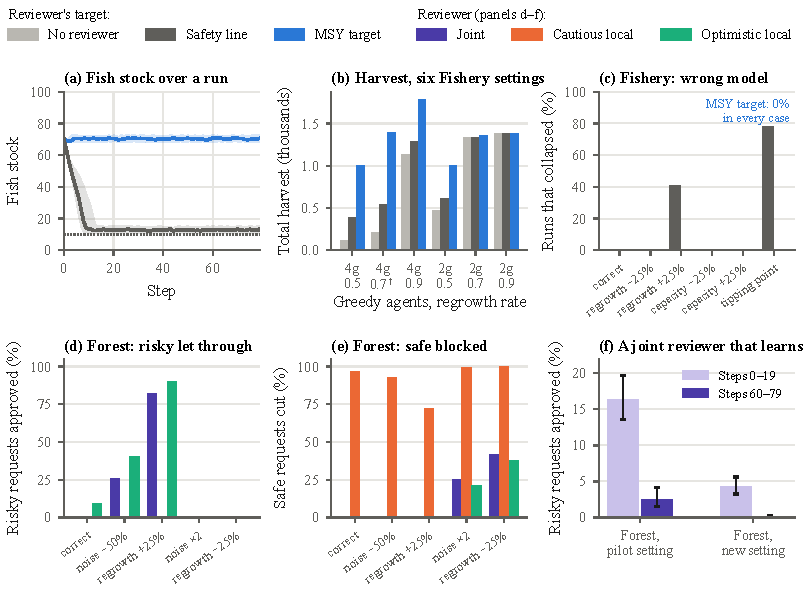
\includegraphics[width=0.9\textwidth]{../figures/fig2_reviewer.pdf}
  \caption{What the reviewer aims for and what it knows. Top row, \game{Fishery}: stock over one run under the one-step line and the half-capacity target; total harvest in six settings; collapses when the reviewer's model is wrong. Bottom row, \game{Forest}: risky requests let through and safe requests blocked when part of the reviewer's model is wrong, and a reviewer that learns the model while running. Error bars: 95\% intervals.}
  \label{fig:reviewer}
\end{figure}

\begin{table}[h]
  \centering\small
  \caption{Audit rules compared (\game{Fishery}, half-capacity target, 64 new populations). Bold: best in column.}
  \label{tab:regimes}
  \resizebox{0.95\textwidth}{!}{\begin{tabular}{llrrrr}
\toprule
Audit rule & Audit rate $q$ & Cheaters' extra harvest [95\% interval] & Harvest per honest agent & Steps over MSY limit (\%) & Checks per step \\
\midrule
No audits & --- & 112.8 [106, 120] & 39.5 & 100 & 0.00 \\
\addlinespace[2pt]
Fine & 0.10 & \textbf{0.0} & \textbf{104.1} & \textbf{0} & 0.61 \\
 & 1/6 & \textbf{0.0} & \textbf{104.1} & \textbf{0} & 1.00 \\
\addlinespace[2pt]
Lower allowance for caught agents & 0.10 & 58.4 [49, 68] & 74.5 & 54 & 0.61 \\
 & 1/6 & 55.1 [46, 65] & 77.1 & 49 & 1.00 \\
\addlinespace[2pt]
Check caught agents every round & 0.10 & $-$3.5 [$-$36, 14] & 95.2 & 16 & 3.78 \\
 & 1/6 & 8.3 [7, 10] & 99.4 & 10 & 4.07 \\
\addlinespace[2pt]
Lower allowance for all agents & 0.10 & 141.7 [136, 147] & 36.0 & 24 & 0.61 \\
 & 1/6 & 142.3 [137, 148] & 36.0 & 16 & 1.00 \\
\addlinespace[2pt]
Fine and lower allowance for all agents & 0.10 & \textbf{0.0} & \textbf{104.1} & \textbf{0} & 0.61 \\
 & 1/6 & \textbf{0.0} & \textbf{104.1} & \textbf{0} & 1.00 \\
\midrule
Nobody cheats & --- & 0 & 104.1 & 0 & 0 \\
\bottomrule
\end{tabular}
}
\end{table}

\subsection*{D\quad How the LLM agents over-take (post hoc)}
\begin{figure}[h]
  \centering
  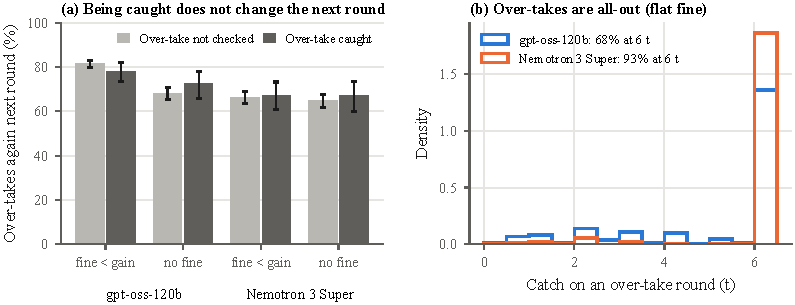
\includegraphics[width=0.85\textwidth]{../figures/figA1_llm_behaviour.pdf}
  \caption{Post hoc analyses of gpt-oss and Nemotron. (a)~After an over-take, the chance of over-taking again barely depends on whether the agent was caught. (b)~Over-takes are mostly at the 6\,t maximum. Intervals over agent-rounds, which are not independent; descriptive only.}
  \label{fig:a1}
\end{figure}

\subsection*{E\quad Protocols and reproducibility}
Each study had a protocol frozen before its code, with hypotheses, falsifiers, sample sizes and analyses; amendments are dated and state what had been seen. The LLM studies used six amendments (an output-parsing fix; remote execution; a held-back and corrected memory cell; the replacement of Mistral Large 4, which used about 6{,}000 hidden-reasoning tokens per decision, by Mistral Large 3; and two infrastructure fixes) and one note that partial results of the threshold test were seen during the run, with nothing changed. Code, protocols, prompts, every game and all analysis scripts will be released.

\end{document}
